\documentclass[twocolumn]{jsarticle}
\usepackage[dvipdfmx]{graphicx}
\usepackage{fancyhdr}
\pagestyle{fancy}
\renewcommand{\headrulewidth}{0pt}
\renewcommand{\footrulewidth}{0pt}
\usepackage{url}
\usepackage{fancyvrb}

\setlength\intextsep{0pt}
\setlength\textfloatsep{-5pt}

\usepackage{setspace}

\fancyhead[L]{神奈川大学理学部}
\fancyhead[C]{情報科学科}
\fancyhead[R]{馬谷研究室}
\fancyfoot[C]{}


%% 論文タイトル
\title{\textbf{Schemeサブセットの操作的意味論のRedexによる実装}}
%% 氏名 学籍番号
\author{武田 雄一郎 201803709}
\date{} % この行も書き換えない(空白のまま)

\begin{document}
\maketitle
\thispagestyle{fancy}

\section{はじめに}


抽象解釈器の構築においてScheme言語派生のRacket言語のライブラリであるRedexを用いる.
Redexとは文法と簡約関係を記述し定義する事で実行可能な仕様を作成するライブラリである.

Redexを用いる利点は,\verb|traces|機能を用いることで簡約の各ステップを簡約グラフを使って網羅的に可視化できることである.

最終的にはSchemeサブセット\cite{3}を基にした抽象解釈器の構築をSchemeサブセットのRedexによる実装,継続データのヒープ化\cite{4},ヒープ化したデータ構造の有限化\cite{5}という手順により行う.本研究ではこれら手順の一つ目であるSchemeサブセットのRedexによる実装を行う.
\section{背景}
抽象解釈とはプログラムを抽象化によって単純化し近似的に実行してプログラムの解析を行うことである.プログラムを近似的に実行することで
不必要な部分を無視し必要な結果だけを部分的に求めることができるため効率的にプログラムの解析を行うことができる.

例えば,符号解析の場合$3$と$-100$という数値を符号に抽象化した場合その符号は$3$は$(+)$,$-100$は$(-)$となる.

また,数値で計算をしてからその符号の結果を確認する通常の解釈とは違い抽象解釈は符号だけで計算する.
$3+(-100)=(-97)$を抽象解釈を用いて計算すると$(+)+(-)=(+/0/-)$となる.ここで,$(+)$は正の抽象値,$(-)$は負の抽象値,$(+/0/-)$は正,ゼロ,負のどの場合もあり得る抽象値を表す.
\section{文法と簡約定義}
本章ではSchemeサブセット\cite{3}のRedexによる実装を行う上でRedexの使用方法について説明する.

まず,Schemeサブセットの文法を正確に定義するために\verb|define-language|形式で文法を使用する.
\begin{verbatim}
(define-language SCM
(p (store (sf ...) e))
(sf (x v))
(e (e e ...)
  (set! x e) 
  (begin e e ...)
  (if e e e) 
  x
  v)
(v (lambda (x ...) e)
    n  #t #f - unspecified)
     /*省略*/
\end{verbatim}  
\verb|p|は変数\verb|x|から値\verb|v|をマッピングする\verb|store|と式\verb|e|で構成され,プログラムの実行状態を表す.
\verb|sf|は\verb|store|中のフィールドで,変数\verb|x|に値\verb|v|が格納されていることを表す.
\verb|e|は関数呼び出し,\verb|set!|式,\verb|begin|式,\verb|if|式,変数\verb|x|,値\verb|v|を表す非終端記号である.
\verb|v|はラムダ式,数値\verb|n|,ブール値,否定演算子,\verb|unspecified|という値を表す.

簡約関係は\verb|reduction-relation|を用いて定義する.簡約関係の形式は言語名,与えられた領域,\verb|-->|で示されたいくつかの節で定義され,左辺,右辺, 任意の数の\verb|side condition|,任意の名前からなり一連の書き換え規則を受け取り二項関係を定義する.

\verb|SCM|の簡約関係\verb|rS|を以下のように定義する.全部で7つある規則のうち,ここでは2つだけを示す.
\begin{verbatim}
(define rS
(reduction-relation
SCM #:domain p
(-->
  (store (sf_1 ... (x_1 v_1) sf_2 ...)
         (in-hole E (set! x_1 v_2)))
  (store (sf_1 ... (x_1 v_2) sf_2 ...)
         (in-hole E  100))
  "Mset")
(-->
  (store (sf_1 ... (x_1 v_1) sf_2 ...)
         (in-hole E x_1))
  (store (sf_1 ... (x_1 v_1) sf_2 ...)
         (in-hole E v_1))
  "Mlookup")))
\end{verbatim}
\verb|P|,\verb|E|は,それぞれ\verb|p|,\verb|e|中の簡約可能箇所が穴になっている文脈である.

1つ目の\verb|Mset|規則とは関連する値をストア内の指定された識別子を指定された置換文字列で置き換える規則である.2つ目の\verb|MLookup|規則とは,変数の評価に対応しており,変数を\verb|store|内の関連する値に置き換える規則である.

このようにRedexを用いるには文法と簡約関係を定義する必要がある.
\section{実行例}
\begin{verbatim}(store ((x 1) (y 3) (z 5))
 ((set! x y) (set! x z)))\end{verbatim}を3章で定義した文法,簡約関係から\verb|traces|機能を用いて以下のコードを実行する.
\begin{verbatim}
> (traces rS 
   (term (store ((x 1) (y 3) (z 5))
   ((set! x y) (set! x z)))))
\end{verbatim}
実行した結果,図1のように簡約グラフが表示される.
\begin{figure}[t]
    \centering
    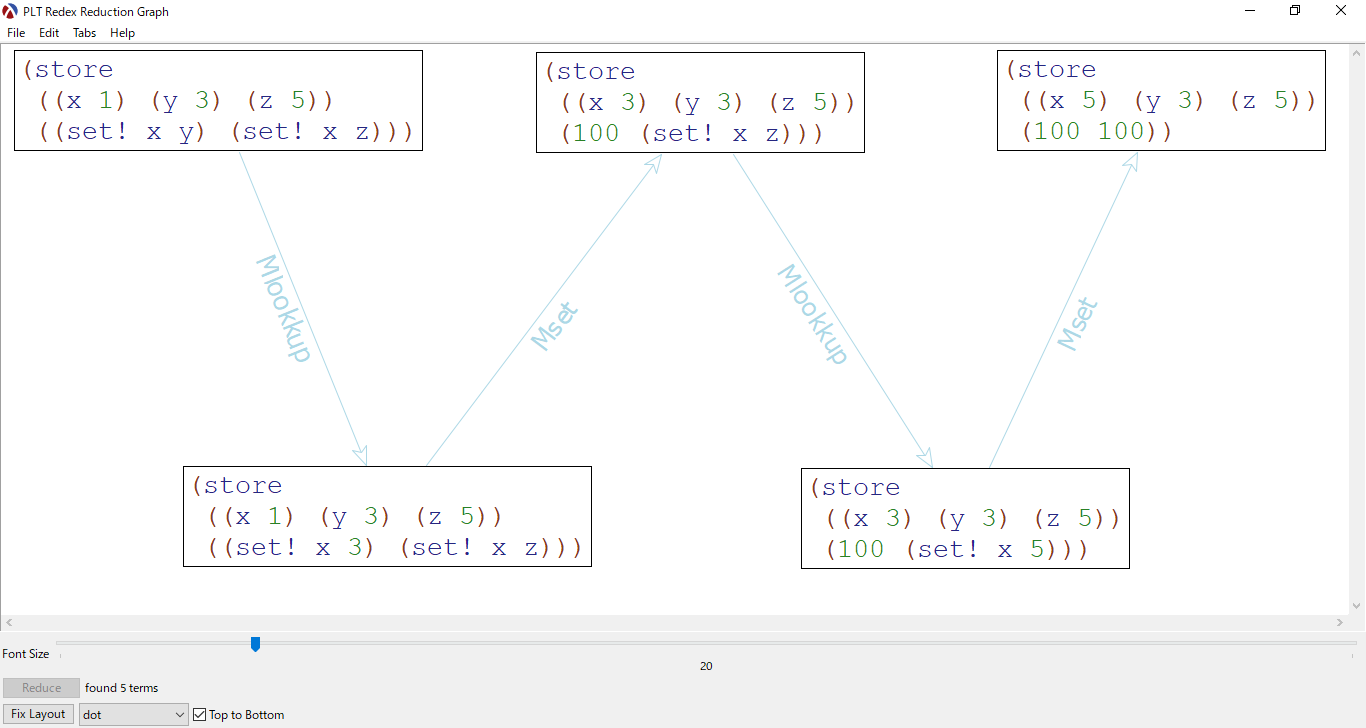
\includegraphics[scale=0.2]{redex.png}
    \caption{Redexによる簡約グラフの可視化}
    \label{fig:latticemix}
\end{figure} 
図1の簡約グラフから\verb|SCM|の簡約関係を正しく定義できていることが確認できる.
\section{まとめ}
本研究ではSchemeサブセットのRedexによる実装を行った.
Schemeサブセットを基にした抽象解釈器の構築においてRedexによる実装が本研究により可能であることを確認した.
\begin{thebibliography}{99}
\bibitem{1}Robert Bruce Findler,Casey Klein,Burke Fetscher,Matthias Felleisen,Redex: Practical Semantics Engineering.\url{https://docs.racket-lang.org/redex/index.html}
\bibitem{2}David Van Horn, An Introduction to Redex with Abstracting Abstract Machines (v0.6). \url{https://dvanhorn.github.io/redex-aam-tutorial/}
\bibitem{3}Jacob Matthews,Robert Bruce Findler,An Operational Semantics for Scheme,Journal of Functional Programming, 18(1), 47--86,2007.
\bibitem{4}山本怜,Redex 上の Scheme インタプリタにおける抽象解釈のための継続のヒープ化,2021年度神奈川大学理学部情報科学科卒研要旨集,2022.
\bibitem{5}森田翔大,Redex 上のScheme インタプリタにおけるヒープの有限化による抽象解釈の実現,2021 年度神奈川大学理学部情報科学科卒研要旨集,2022.
\end{thebibliography}

\end{document}
